\chapter{\textsc{Implementación de los circuitos en lenguaje de descripción de hardware} }\label{implementaciónHDL}
\section{Introducción}
Utilizamos un lenguaje de descripción de \emph{hardware} (\gls{hdl} por su sigla en inglés) para implementar los distintos circuitos que evaluaremos, porque el problema planteado en el capítulo \ref{chap:especificaciones}, requiere que podamos crear un sumador de $n$ bits arbitrario, para lo cuál los HDL son la herramienta mas apropiada. Implementarlos por medio de esquemáticos llevaría mucho tiempo, por eso descartamos esa metodología. En cambio, cuando describimos un circuito con un HDL lo hacemos parametrizando el tamaño del mismo, y a la hora de simularlo o implementarlo físicamente, determinamos su tamaño y generamos automáticamente el circuito. 

\subsection{Breve reseña de los \gls{hdl}}
\gls{vhdl} y Verilog son los lenguajes más utilizados y conocidos para el diseño de circuitos integrados. \gls{vhdl} nace como lenguaje de documentación del comportamiento de los circuitos integrados de aplicación específica\footnote{Conocido comunente como \gls{asic}}. El departamento de defensa de Estados Unidos lo desarrolló para poder especificar a sus proveedores, cómo debía comportarse el sistema digital que les encargaba diseñar. Luego, surgio la idea de realizar una simulación lógica a partir de estos archivos \gls{vhdl}. Lo siguiente fué el desarrollo de herramientas de síntesis lógica a partir de estos archivos, para generar una implementación física del circuito. Con Verilog sucedió algo muy parecido, aunque dentro del ámbito de la industria. Por esta historia en común, se puede decir que estos dos lenguajes tienen varias finalidades, siendo la implementación en \emph{hardware} tan sólo una de ellas, es decir, uno puede describir circuitos que no son sintetizables. Por esa razón, y a pesar de ser los más utilizados y conocidos para describir circuitos digitales, no siempre son la mejor alternativa a elegir.

\subsection{Nuevos \gls{hdl}s}\label{subsec:nuevosHDL}
Podemos mencionar al menos tres lenguajes de descripción de \emph{hardware} que están siendo utilizados para el diseño de circuitos integrados, que nacieron con el objetivo de aprovechar las ventajas de nuevos lenguajes de programación, bajo el paradigma de la programación funcional. Estos son, \textbf{Lava}\cite{Lava} y \negrita{C$\lambda$aSH}\cite{Clash} basados en \textbf{Haskell}, y \textbf{Chisel}\cite{Chisel}, basado en \textbf{Scala}. En este tipos de lenguajes, un circuito que no sea sintetizable es un error de sintáxis. 

Otro lenguaje que queremos mencionar es \textbf{MyHDL}\cite{MyHDL}, un lenguaje basado en Python que brinda muchas ventajas de este lenguaje, que por estar basado en otro paradigma de programación, no lo agrupamos con los cuatro anteriores. Pero estos cinco lenguajes nos permiten:

\begin{itemize}
\item Usar un único lenguaje para describir (con distintos niveles de abstracción), simular, verificar e implementar el circuito.
\item Los circuitos se describen en Haskell, Scala o Python (según correspoda), el HDL es simplemente un conjunto de módulos que permiten realizar nuevas tareas relacionadas al diseño de \emph{hardware}, como puede ser crear un netlist \gls{vhdl}, simulación simbólica, etc. 
\item Generar automáticamente una descripción en \gls{vhdl} o Verilog, lo cuál nos permite utilizar herramientas de diseño físico que usan este tipo de lenguajes como entrada.
\item Describir circuitos que construimos a partir de subcircuitos, además de la posibilidad de reutilizar fácilmente patrones de conexión.
\end{itemize}

\subsection{¿Por qué Lava?}
Podemos elegir arbitrariamente cualquiera de estos lenguajes, ya que el circuito que lograremos es independiente del lenguaje utilizado. Por lo tanto, para este proyecto en particular\footnote{Es un circuito puramente combinacional} se puede elegir el HDL basado en el conocimiento y experiencia de uso en Haskell, Python o Scala.

Para describir el circuito, elegimos Lava. Quien haya utilizado alguna vez un lenguaje de programación funcional, entenderá fácilmente cómo describir circuitos. Quien no conozca este paradigma de programación, podrá aprender a utilizar Lava por medio de su documentación\cite{Lava-tutorial} sin muchas dificultades, ya que el paradigma de programación se basa en definir a los programas como se definen las funciones matemáticas. En Lava los circuitos son descriptos como funciones que operan sobre listas, tuplas o sobre circuitos. Esto último se debe a que el lenguaje Haskell permite la definición de funciones de alto orden, es decir podemos definir funciones que su dominio e imagen son funciones. 

Lava es simplemente un conjunto de módulos de Haskell, por lo tanto estamos unificando un conjunto de tareas del diseño digital utilizando un lenguaje de programación de propósito general. Las ventajas de este acercamiento al diseño son varias: 

\begin{itemize}
\item Disponibilidad de todas las librerías existentes en Haskell para ampliar las posibilidades de nuestra herramienta.
\item No se generan \cursi{bugs} típicos de implementar dos veces el mismo circuito en dos lenguajes de programación distintos: El primero en la implementación a nivel de sistema y el otro a nivel de \cursi{hardware}.
\item Se pueden aplicar técnicas de programación propias del lenguaje como \cursi{testing} o \cursi{model checking} con el circuito.
\item Permite manejar otros programas externos, por ejemplo lanzamos \negrita{minisat}\cite{minisat} para verificar formalmente nuestro circuito.  
\end{itemize}


Con la implementación del circuito utilizando este HDL, podemos generar un \negrita{netlist} \gls{vhdl}, hacer simulación digital, verificación formal de propiedades, y la ventaja de  


\section{Implementación en lenguaje de descripción de hardware}
Ya hemos presentado una descripción esquemática del sumador binario de \(n\) bits en la figura \ref{fig:RCA} y en la \ref{fig:bkungadder}. El objetivo es implementar estos circuito en Lava parametrizando el tamaño \(n\) de los sumandos. 

\subsection{Implementación del sumador de \textbf {ripple carry} en Lava}

\noindent Siguiendo la figura \ref{fig:halfadder}, definiremos el semisumador:
\begin{lstlisting}
halfAdd (a, b) = (s, c)
   where
      s = xor2 (a, b)
      c = and2 (a, b)
\end{lstlisting}
\noindent Para escribir el circuito del sumador completo usamos la figura \ref{fig:fulladder}, nombrando las señales internas y 
escribiendo los subcomponentes de la siguiente forma:
\begin{lstlisting}
fullAdd (cin, (a, b)) = (s, cout)
    where
       (sum1, carry1) = halfAdd (a, b)
       (s   , carry2) = halfAdd (cin, sum1)
       cout           = xor2 (carry2, carry1)
\end{lstlisting}

Por último escribimos la descripción del sumador binario (RCA) de la figura \ref{fig:RCA} de la siguiente forma:

\begin{lstlisting}
rcAdder (carryIn, ([], []))     = ([], carryIn)
rcAdder (carryIn, (a:as, b:bs)) = (sum:sums, carryOut)
   where
      (sum, carry)     = fullAdd (carryIn,(a, b))
      (sums, carryOut) = rcAdder (carry, (as, bs))
\end{lstlisting}

\subsection{Patrones de conexión}
\paragraph{Patrones de conexión estandars.} Los patrones de conexión son funciones de alto orden\footnote{Las funciones de alto orden (\emph{high order functions}) son funciones que toman otras funciones como argumento y devuelven otra función como resultado.} que pueden ser utilizadas para construir circuitos, les llamamos circuitos de alto orden o generadores de circuitos.

\begin{figure}[h]
  \centering
\hspace{-23pt}
%[width=\textwidth]
\begin{subfigure}[b]{0.45\textwidth}
                \centering
                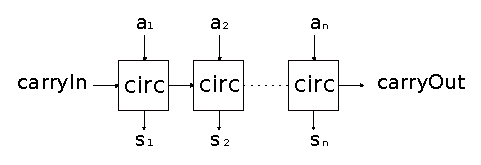
\includegraphics[scale=0.9]{figuras/rowCirc.eps}
                \caption{row}
                \label{fig:rowcirc}
        \end{subfigure}
\begin{subfigure}[b]{0.25\textwidth}
                \centering
                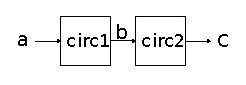
\includegraphics[scale=1]{figuras/serial.eps}
                \caption{serial}
                \label{fig:serial}
        \end{subfigure}
\begin{subfigure}[b]{0.30\textwidth}
                \centering
                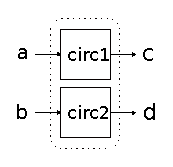
\includegraphics[scale=1]{figuras/par.eps}
                \caption{parallel}
                \label{fig:parallel}
        \end{subfigure}
  \caption{Diferentes patrones de conexión de circuitos}\label{fig:pattern}
\end{figure}


Observando la definición de {\footnotesize\verb|rcAdder|} y su topología, podemos generalizar esa estructura de conexión reemplazando el circuito por un parámetro, que en la definición\footnote{Esto es posible dado que Haskell implementa \emph{pattern matching}.} del circuito será una entrada mas. A ese parámetro lo nombramos {\footnotesize\verb|circ|}:

\begin{lstlisting}
row circ (carryIn, ([])) = ([], carryIn)
row circ (carryIn, a:as) = (b:bs, carryOut)
   where
      (b, carry)     = circ (carryIn, a)
      (bs, carryOut) = row circ (carry, as)
\end{lstlisting}

La función {\footnotesize\verb|row|} toma un circuito {\footnotesize\verb|circ|}, un conjunto de entradas, y las conecta como se muestra en la figura \ref{fig:rowcirc}. Ahora, usando el generador de circuito {\footnotesize\verb|row|}, el sumador binario lo podemos describir mas simplemente asi:
{\footnotesize
\begin{verbatim}
rcAdder' (carry, inps) = row fullAdd (carry, inps)
\end{verbatim}
}
Inclusive para simplificar mas, podemos currificar\footnote{Currificar, es una referencia al lógico Haskell Curry, y hace referencia a la técnica que consiste en transformar una función que utiliza una n-tupla como argumento, en una función que utiliza un único argumento.} la definición:
{\footnotesize
\begin{verbatim}
rcAdder'' = row fullAdd
\end{verbatim}
}

Definir {\footnotesize\verb|rcAdder'|} y {\footnotesize\verb|rcAdder''|} de esa forma es bastante conveniente ya que podemos pensar en término de \emph{generadores de circuitos} en vez de recursión sobre listas.

Ya que hemos visto la ventaja de definir los patrones de conexión, presentamos dos generadores de circuitos que vamos a usar mas tarde:

{\footnotesize
\begin{verbatim}
par cir1 cir2 (a, b) = (c, d)
   where
      c = cir1 a
      d = cir2 b
\end{verbatim}
}
Es muy útil definir una versión mas gráfica de la función {\footnotesize\verb|par|}, si definimos el operador infijo {\footnotesize \verb1-|-1}:
{\footnotesize
\begin{verbatim}
cir1 -|- cir2 = par cir1 cir2 
\end{verbatim}
}
Y por último la conexión serie y su versión con el operador infijo:
{\footnotesize
\begin{verbatim}
serial cir1 cir2 a = c
   where
      b = cir1 a
      c = cir2 b
\end{verbatim}
}
{\footnotesize
\begin{verbatim}
cir1 ->- cir2 = serial cir1 cir2
\end{verbatim}
}
\subsection{Sumador de Brent-Kung}
\subsubsection {Operador de Brent-Kung}
\noindent Comencemos a describir el sumador de Brent-Kung.
En Lava, podemos describir el circuito que implementa la función \ref{gap} siguiendo la figura \ref{dotOp}:

\begin{lstlisting}
dotOp ((g1, p1) ,(g, p)) = (go, po)
   where
      go = or2 (g, and2 (p, g1))
      po = and2 (p, p1)
\end{lstlisting}

\subsubsection {Generación y Propagación del Acarreo}
\noindent En Lava escribimos asi lo que captamos de la figura \ref{gAndPs}:
\lstset{language=Haskell}
{
\begin{lstlisting}
gAndPs ([],[]) = []
gAndPs (a:as, b:bs) = (g,p):gps
   where
      (g, p) = (and2 (a, b),xor2 (a, b))
      gps    = gAndPs (as, bs)
\end{lstlisting}
}


Para ver una explicación con mayor nivel de detalles de cómo construir el circuito, ver el manual de Lava \cite{Lava-tutorial} en conjunto con el paper aqui citado \cite{4638988}


\subsubsection {Red de Prefijos Paralelos para el sumador de Brent-Kung}
\noindent Ahora para describir esta red que usamos en la figura \ref{fig:bkungadder} y mostramos un ejemplo de una red para 16 bits en a figura \ref{bKung16}, nos basamos en un patrón recursivo que propone Sheeran \cite{Shee07} al que le llama \emph{wrap}. En cada paso de la iteración tomamos el resultado anterior (el circuito \(P\)) y le aplicamos el operador punto antes y después de forma intercalada como se puede ver en la figura \ref{sheeranrecurrence}. Esto nos lleva a construir redes como la de la figura \ref{bKung16}.


\begin{figure}[h!]
\centering
 \begin{subfigure}{0.4\textwidth}
    \centering
    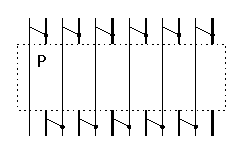
\includegraphics[scale=2.2]{figuras/sheeranrecurrence.eps}
%\vspace{0.05cm}
    \caption{Patrón de recurrencia}
    \label{sheeranrecurrence}
 \end{subfigure}
 \begin{subfigure}{0.5\textwidth}
    \centering
    
\includegraphics[scale=1.92]{figuras/wrapR.eps}
    \caption{Primeras iteraciones de ppNet}
    \label{firstsiter}
 \end{subfigure}
 \caption{Construcción de la red de prefijos paralelos de Brent-Kung.}
\end{figure}


La figura \ref{firstsiter} representa las dos primeras iteraciones del circuito \verb|ppNet|, en el cual la caja de lineas punteada es el caso base de la descripción, los puntos negros son la función \verb|dotOp|. Lo que producimos con esta función recursiva son redes como la de la figura \ref{bKung16}.

A continuación, describimos el circuito \verb|ppNet|, pero antes escribimos las funciones auxiliares \verb|dop|, \verb|unzipl|, \verb|zipl|, \verb|comb|, \verb|posComb|, \verb|miti| y \verb|wrap|, que nos servirán para escribir \verb|ppNet|:


%abss era abs, pero lo renombré xq latex lo resaltaba como una función.
\begin{lstlisting}
dop [a, b] = [a, dotOp(a, b)]
--
unzipl []        = ([],[])
unzipl [a]       = ([a], [])
unzipl (a:b:abss) = (a:as, b:bs)
   where
      (as, bs) = unzipl abss
--
zipl ([], [])     = []
zipl ([a], [])    = []
zipl (a:as, b:bs) = a:b:zipl(as, bs)
--
-- La forma en que hemos escrito las funciones zipl y unzipl 
-- son la clave para lograr una descripcion de un sumador 
-- binario que acepte cualquier cantidad de entradas
--
comb []     = []
comb [a]    = []
comb (a:as) = dop [a, head as] ++ comb (tail as)
--
posComb (a:as)  = a: (comb (init as))++ [last as]
--
miti p = unzipl ->- (id -|- p) ->- zipl
--
wrap p = comb ->- miti p ->- posComb 
\end{lstlisting}

\noindent Luego finalemente, podemos describir {\verb|ppNet|}:

\begin{lstlisting}
ppNet [a]    = []
ppNet [a, b] = dop [a, b]
ppNet as     = wrap ppNet as
\end{lstlisting}


\subsubsection{Circuito top level}
Ahora que ya tenemos construidas todas las partes del sumador, sólo resta juntarlas siguiendo el esquemático de la figura \ref{fig:bkungadder}. Prestar atención a que el circuito \verb|fork| realiza una copia de las señales, el \verb|even| deja pasar los bits pares, \verb|odd| los impares, \verb|id| es la función identidad y \verb|sums| mapea los bits de entrada con la función booleana XOR, salvo el primer y último bit:

\begin{lstlisting}
fork as = (as, as)
--
even as = cs
   where
      (bs,cs) = unzip as
--
odd as = bs
   where
      (bs,cs) = unzip as
-- Unas definiciones mas cortas:
dropP = id -|- odds
dropG = even -|- ppNet
--
sums (a:as,bs) = (a:lastXor (as,init bs),cOut)
   where
      cOut = last bs
--
lastXor (as, bs) = map xor2 cs
   where
      cs = zipp (as, bs)
--
zipp ([],[]) = []

zipp (a:as, b:bs) = c:cs  -- da lo mismo que poner (c:cs)
   where
      c  = (a, b)
      cs = zipp (as, bs)
\end{lstlisting}

\noindent Y el circuito completo es:
\begin{lstlisting}
fastAdd = gAndPs ->- fork ->- dropG ->- dropP ->- sums
\end{lstlisting}


\subsection{Sumador de Sklansky}
En el apéndice \ref{chap:sklansky-lava} brindamos la descripción en Lava del sumador.


\subsection{Simulación}
En Lava podemos simular el circuito usando la operación {\footnotesize\verb.simulate.}, el circuito y el estado de las entradas, por ejemplo:

{\footnotesize
\begin{verbatim}
simulate fastAdd ([high,low],[low,high])
\end{verbatim}
}

\noindent devuelve:{\footnotesize \verb|([high,high],low)|}. También podemos simular secuencia de entradas con la operación {\footnotesize\verb|simulateSeq|}:

{\footnotesize
\begin{verbatim} 
simulateSeq halfAdd [(low,low),(high,low),(low,high)]
\end{verbatim}
}

\noindent que devuelve {\footnotesize\verb|[(low,low),(high,low),(high,low)]|}

\subsubsection{Simulaciones con números enteros en base diez}
Lava nos permite una interfase con números enteros, por si nos interesa simular utilizando esta representación numérica en vez de la binaria. Esto lo logramos si definimos una función como la siguiente, que toma dos enteros y convierte el segundo en un número binario de la cantidad de bits que indica el primero:
\begin{lstlisting}
int2bin 0 num = []

int2bin n num = (bit:bits)
  where
    (bit, num_) = numBreak num
     bits      = int2bin (n-1) num_
\end{lstlisting}

\subsubsection{Método de validación del hardware}
Para este diseño en particular, no utilizaremos la simulación como una forma de validar el correcto funcionamiento del circuito, por eso no avanzaremos en las distintas alternativas de simulación que nos permite el sistema, como puede ser la creación de un archivo VCD\footnote{\gls{vcd} es un formato basado en ASCII para loguear señales, que es utilizado por herramietas de simulación lógica. Para visualizarlo podemos utilizar el software GTKWave, de licencia libre.} a partir de vectores de entrada\footnote{Podemos usar una libreria de Haskell llamada \cursi{vcd} que nos permite escribir y leer archivos con este formato.}.

Justificamos descartar la simulación como método de validación por la simple razón de que sólo simulando todos los posibles estados de las entradas se garantiza el correcto diseño del circuito. Por ejemplo, para un sumador de 64 bits, es necesario simular $2^{128}$ estados.

Para este tipo de sistemas es aplicable la verificación formal automática, que desarrollaremos en el capítulo \ref{verificacion}.

\subsection{Síntesis del \cursi{netlist} \gls{vhdl}}

Para continuar en nuestro flujo de diseño, precisamos generar el circuito en un lenguaje que nuestra herramienta de \emph{Place and Route} pueda manejar. Para eso Lava nos permite crear un netlist \gls{vhdl} siguiendo dos pasos, el primero definiendo los nombres de los puertos y el bloque a ser creado:
\begin{lstlisting}
fastAdder n = writeVhdlInputOutputNoClk
              "BrentKungFastAdder" fastAdd
              (varList n "a", varList n "b")
              (varList n "sum", var "cout")
\end{lstlisting}

Y el segundo paso para crear el netlist, debemos especificar el valor real de sumador, por lo tanto valuamos el circuito con en número de bits del sumador y conseguiremos el archivo BrentKungFastAdder.vhl que mostramos en el apéndice \ref{vhdlNetlist}:
\begin{lstlisting}
Main> fastAdder 16
Writing to file "BrentKungFastAdder.vhd" ... Done..
\end{lstlisting}

\noindent Si por alguna razón este netlist lo utilizaramos con una otra herramienta de síntesis, deberemos especificar que no modifique los cables para preservar la estructura de esta red.

